\chapter{CPU}

\section{流水线结构}

\subsection{总体架构}

CPU采用五级流水顺序双发射架构,分别为取指、译码/发射、执行、访存、写回五级,在较多情况下可以同时发射两条相邻的指令;创新性使用译码级判断数据前递方案,执行级得到前递数据的方法来解决数据冲突。

\begin{figure}[htbp]
	\centering
	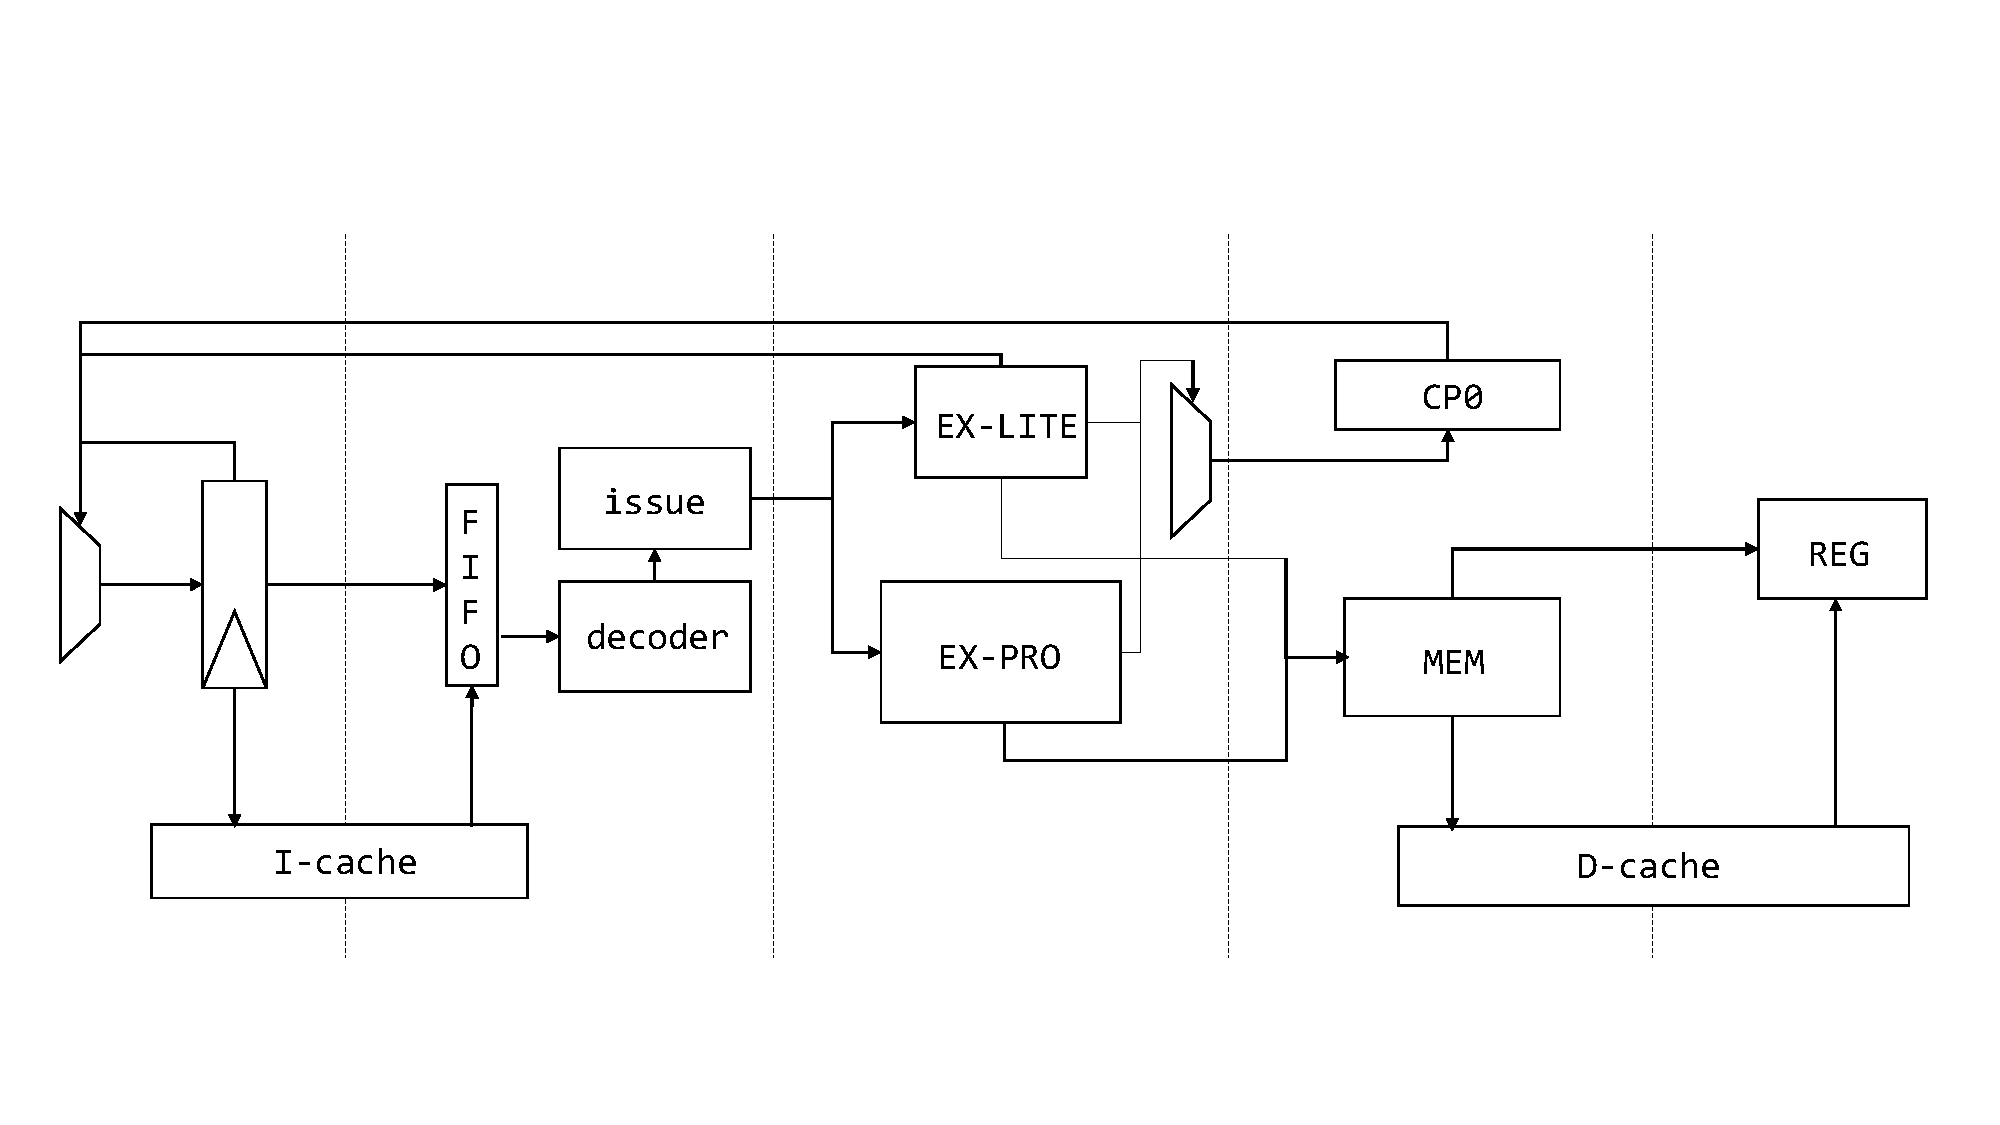
\includegraphics[width=\linewidth]{pipeline.pdf}
	\caption{流水线结构}
	\label{fig:pipeline}
\end{figure}

\subsection{取指级}
取指阶段根据内存管理单元(MMU)给出的cached属性向指令缓存发起取指请求或直接向RAM发起取指请求,每次最多可返回两条指令,并被送入指令FIFO中等待译码阶段取出并发射。

指令FIFO长度为16,采用双指针环形FIFO结构,双指针分别为读指针和写指针。当读指针和写指针指向同一个区域,则当前FIFO为空;当写指针加一为读指针,则当前FIFO为满。当清空流水线、发生分支,将读指针指向写指针。

\subsection{译码/发射级}
该阶段首先从指令FIFO中取出两条指令进行译码,同时会将这两条指令需要读取的寄存器编号送入寄存器文件,寄存器文件将返回数据前递方案(详细见2.2.1数据前递方案)和寄存器文件中对应的寄存器值。此处定义非乘除法的算术运算、逻辑运算指令为简单运算指令;定义数据相关为相邻两条指令的写后读数据相关。

两条流水线分别定义为PRO流水线和LITE流水线,PRO流水线实现了除了分支指令功能外的所有指令共功能;LITE流水线实现了分支指令功能和简单运算指令功能。

发射规则如下:

\begin{enumerate}
    \item 分支和延迟槽始终一起发射,发射方法为将分支发射到LITE流水线,将延迟槽发射到PRO流水线;
    \item 若两条指令中任一条是简单运算指令,且无数据相关,所需寄存器值可在执行阶段获得,则可同时发射两条,发射方法为将其中的简单运算指令发射到LITE流水线,将另一条发射到PRO流水线;
    \item 若只能从FIFO读出一条指令,或两条指令中均非简单运算指令,或两条指令存在数据相关,或第二条指令所需寄存器值不能在执行阶段获得,仅发射第一条,发射方法为将第一条指令发射到PRO流水线;
    \item 若只能从FIFO读出零条指令,或第一条指令所需寄存器值不能在执行阶段获得,发射零条。
\end{enumerate}

为了方便发射逻辑判断,译码得到的指令操作码采用“三位指令类型+五位类型内编号”格式,发射时判断前三位即可得知对应的指令类型。

发射时将有一位标志位reverse表示发射顺序,当reverse为1,代表LITE流水线中的指令是PRO流水线中的指令的前一条;反之,代表PRO流水线中的指令是LITE流水线中的指令的前一条。该标志位将随流水线流水至最后一级。

\subsection{执行阶段}
执行阶段对所有非访存指令进行计算并得到结果,其中乘法指令和除法执行使用Xilinx IP核实现,分别在4个周期和34个周期后返回,执行乘除法指令时会暂停流水线直至计算结果完成。

执行阶段对访存指令进行数据准备,包括访存地址和写入数据的计算等,将虚地址发送给内存管理单元,得到访存的cached属性。

执行阶段对异常进行判断,并仲裁两条流水线的异常情况,最多向异常处理模块提交一个异常和一个CP0寄存器写请求。

执行阶段提交分支请求,由于分支仅在LITE流水线中处理,所以此时不需要仲裁。

\subsection{访存阶段}
访存阶段根据内存管理单元(MMU)给出的cached属性向数据缓存发起访存请求或者直接向RAM发起访存请求。若不能在下一拍完成访存请求,则需要暂停流水线,等待数据返回。

同时在本级处理中断和异常。

\subsection{写回阶段}
写回阶段从获得加载类指令的写回结果和其他所有指令的写回结果,发起寄存器写请求。

\subsection{级间数据前递方案}
本项目创新性地使用译码阶段、执行阶段相配合的方案进行数据前递。译码阶段获取前递方案,执行阶段根据前递方案获取寄存器的值。

译码阶段在从FIFO取出两条指令后向寄存器文件模块发送指令中的rs,rt寄存器编号,寄存器文件根据当前执行阶段和访存阶段的指令的写寄存器情况确认前递方案。每个寄存器的前递方案采用4位表示,分别代表使用执行阶段PRO流水线的结果、使用执行阶段LITE流水线的结果、使用访存阶段PRO流水线的结果、使用访存阶段LITE流水线的结果。同时对于每个寄存器使用一位有效位表示前递方案是否有效,如果存在访存相关的数据前递,则有效位置为无效。

发射方案和前递方案有关,当一指令某一寄存器的前递方案无效且需要读该寄存器时,需要等待直至该指令的前递方案有效才能发射该指令。

执行阶段根据前递方案,在访存阶段的结果、写回阶段的结果、寄存器文件的数据中做出选择。由于流水线前进一级,前递方案的4位此时分别对应使用访存阶段PRO流水线的结果、使用访存阶段LITE流水线的结果、使用写回阶段PRO流水线的结果、使用写回阶段LITE流水线的结果,如果四位均无效,则选择寄存器文件中的数据。

\subsection{级间控制信号}
取指、译码/发射、执行、访存四级之间均有清空(flush)、暂停(stall)两个控制信号;访存和写回之间有清空(flush)信号。由统一的控制模块接受各级流水的暂停请求和例外请求,继而对各级发出控制信号。

\section{指令集}
CPU在大赛要求的57条指令基础之上,增加了部分指令以启动操作系统。实现的所有指令如下:
\begin{itemize}
	\item \textbf{算术运算指令} ADD, ADDU, SUB, SUBU, ADDI, ADDIU, SLT, SLTU, SLTI, SLTIU, MUL, MULT, MULTU, DIV, DIVU, MADD, MADDU, MSUB, MSUBU, CLO, CLZ
	\item \textbf{逻辑运算指令} AND, OR, XOR, ANDI, ORI, XORI, NOR, LUI
	\item \textbf{移位指令} SLL, SRL, SRA, SLLV, SRLV, SRAV
	\item \textbf{访存指令} SB, SH, SW, SWL, SWR, LB, LBU, LH, LHU, LW, LWL, LWR
	\item \textbf{分支跳转指令} BEQ, BNE, BGEZ, BGTZ, BLEZ, BLTZ, BGEZAL, BLTZAL, J, JAL, JR, JALR
	\item \textbf{数据移动指令} MFHI, MFLO, MTHI, MTLO, MOVZ, MOVN
	\item \textbf{特权指令} CACHE(实现为空), SYSCALL, BREAK, TLBR, TLBWR, TLBWI, TLBP, ERET, MTC0, MFC0, PREF(实现为空), SYNC(实现为空), WAIT(实现为空)
\end{itemize}

\section{协处理器0}
CPU实现了MIPS 32 Rev 1规范中协处理器0中的大部分寄存器,同时为了启动操作系统,实现了MIPS 32 Rev 2规范中的EBase寄存器。所有寄存器如下,名称摘录自参考资料3:
\begin{itemize}
    \item Index Register (CP0 Register 0, Select 0)
    \item Random Register (CP0 Register 1, Select 0)
    \item EntryLo0, EntryLo1 (CP0 Registers 2 and 3, Select 0)
    \item Context Register (CP0 Register 4, Select 0)
    \item PageMask Register (CP0 Register 5, Select 0)
    \item Wired Register (CP0 Register 6, Select 0)
    \item BadVAddr Register (CP0 Register 8, Select 0) 
    \item Count Register (CP0 Register 9, Select 0)
    \item EntryHi Register (CP0 Register 10, Select 0)
    \item  Compare Register (CP0 Register 11, Select 0)
    \item  Status Register (CP Register 12, Select 0)
    \item  Cause Register (CP0 Register 13, Select 0)
    \item  Exception Program Counter (CP0 Register 14, Select 0)
    \item  Processor Identification (CP0 Register 15, Select 0)
    \item  EBase Register (CP0 Register 15, Select 1)
    \item  Configuration Register (CP0 Register 16, Select 0)
    \item  Configuration Register 1 (CP0 Register 16, Select 1)    
\end{itemize}

\section{内存管理}

CPU使用内存管理单元(MMU)来进行虚地址到实地址的转换。对于kseg0和kseg1两段进行直接映射,kuseg、kseg2、kesg3通过转换检测缓冲区(TLB)转换,当转换检测缓冲区(TLB)发生缺失时,触发例外,由软件调入新的TLB项消除例外。
CPU共有8项TLB,为了保证良好时序,设计ibuffer和dbuffer,分别对应指令和数据访存最近使用到的TLB项。当虚地址在kseg0、kseg1或在buffer中,可以在执行级当拍返回实地址;否则,将当拍返回流水线暂停信号,下一拍查找8项TLB,返回实地址或者TLB例外。

\section{中断和异常}
\subsection{中断}
CPU中支持2个软件中断(SW0~SW1)、6个硬件中断(HW0~HW5)和1个计时器中断。其中计时器中断复用HW5硬件中断。

\subsection{异常}
CPU实现了MIPS规范的精确异常,在访存级统一提交异常。CPU中实现的异常如下,名称摘录自参考资料3:
\begin{itemize}
    \item TLB Refill Exception 
    \item TLB Invalid Exception
    \item TLB Modified Exception
    \item Integer Overflow Exception
    \item System Call Exception
    \item Breakpoint Exception
    \item Reserved Instruction Exception
    \item Coprocessor Ununable Exception
    \item Address Error Exception
\end{itemize}

\section{缓存设计}

CPU实现了指令缓存和数据缓存,分别响应CPU取指与访存模块的请求。并且在与AXI的通信中都采用了Wrap模式,能够做到优先返回请求的字。

\subsection{指令缓存 (I-Cache)}

指令缓存能够响应双发CPU的取指请求。CPU在请求缓存时给出一个地址,I-Cache会尽量尝试返回从这一地址开始的连续两条指令。在给出请求的当拍,I-Cache将返回给CPU两条指令的 valid 信号,指示返回的指令条数,然后在下一拍给出对应的指令数据。

I-Cache的参数配置为2路、每路256行、每行8字。I-Cache能够返回已写入缓存的指令以及与AXI通信过程中已经获取到的指令。当连续命中时,I-Cache可以不间断地、流水地返回指令。在发生命中时,会选中需要换出的行,并发起AXI请求从内存中读取缺失的行。在读完这一行的全部数据之后,再用一拍写回。

在I-Cache的工作过程中,除了写回的那一拍之外,都能立即返回在Cache中的、或者已经从AXI接口读取到的指令。I-Cache 使用 AXI Block Memory Genertor 定制的 Naive RAM 作为数据存储单元。

\subsection{数据缓存 (D-Cache)}

\begin{figure}[htbp]
	\centering
	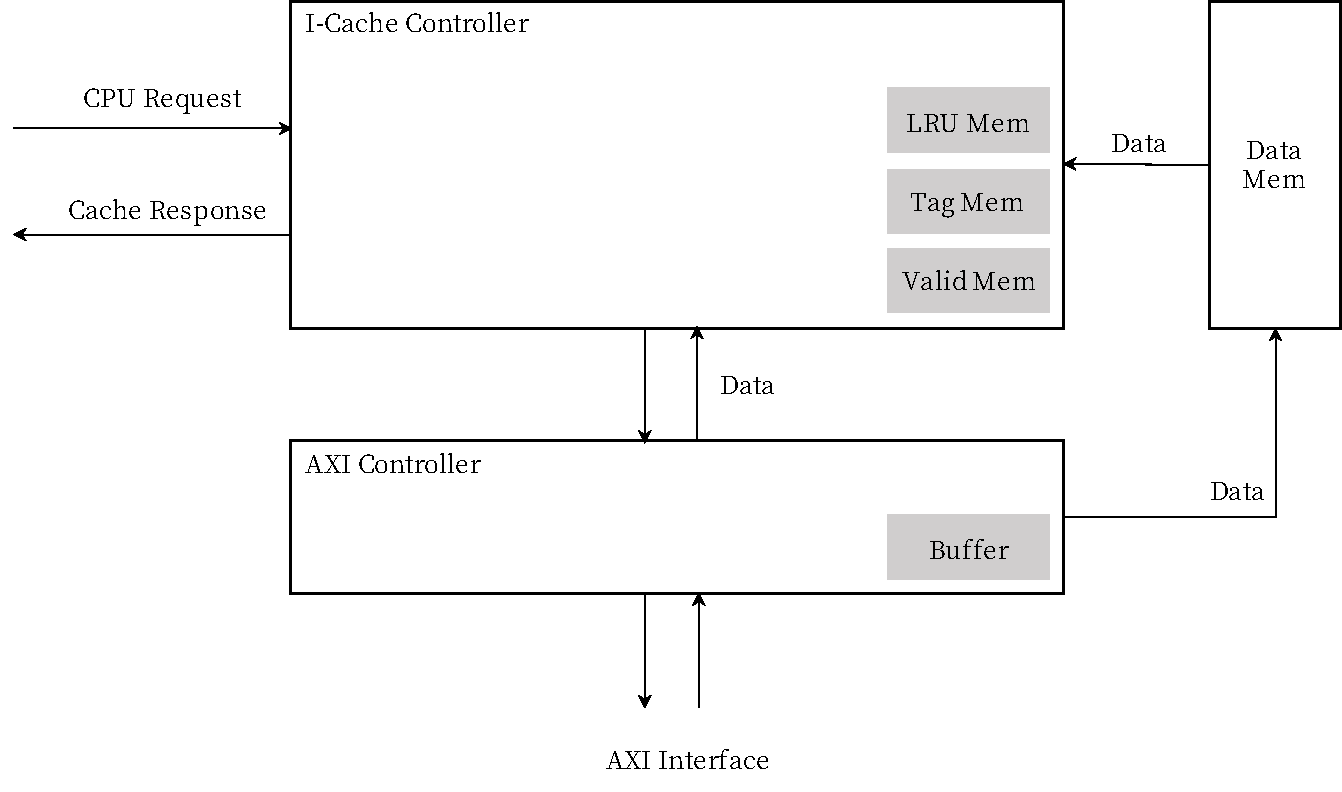
\includegraphics[width=\linewidth]{icache.pdf}
	\caption{I-Cache结构}
	\label{fig:dcache}
\end{figure}

数据缓存能够响应CPU的访存请求。对于CPU发来的请求,D-Cache能够在当拍返回 wait 信号告知CPU是否能完成请求,若是读请求且无需 wait,则会在下一拍给出读取的数据。

D-Cache能够命中缓存的数据以及在AXI读取中已经获得的数据。当连续命中时,D-Cache能够不间断地、流水地完成访存请求。无论是读请求还是写请求,只要命中,D-Cache都能够连续完成请求。

当发生 miss 时,D-Cache将选中需要换出的行,若选中的行需要写回 (dirty 标志位有效),D-Cache会在下一拍从缓存数据中读出这一行,并在下一拍将这一行的数据与地址提交给 Victim Cache,若 Victim Cache 的FIFO没有被充满,则一拍内即可完成提交;同时,D-Cache会向 Victim Cache 发起查询,检查缺失的行是否在其内,若有,则在一拍内读回,若没有,则发起AXI请求,从AXI接口读取缺失的行。当读取到这一行的所有数据后,在一拍内写回。

与 I-Cache 类似,除了写回的那一拍,只要发起的请求命中缓存,D-Cache都能在一拍内完成请求,并且不间断地完成连续命中的请求。

除此以外,D-Cache能够缓存一次发生 miss 的写请求。具体地,当D-Cache得到了CPU发来的一个写请求,发生 miss,且此时AXI控制逻辑空闲时,D-Cache不会阻塞流水线,而是直接拉低 wait 信号,缓存这个请求,开始AXI读,在读到需要的字之后再完成请求。这样的设计能够在单独的写请求发生 miss 时,减少对流水线的阻塞,优化整体性能。

D-Cache的参数配置为2路、每路256行、每行8字。此外,D-Cache由Chisel3开发完成,支持相联度、行数、行大小可配置。

\begin{figure}[htbp]
	\centering
	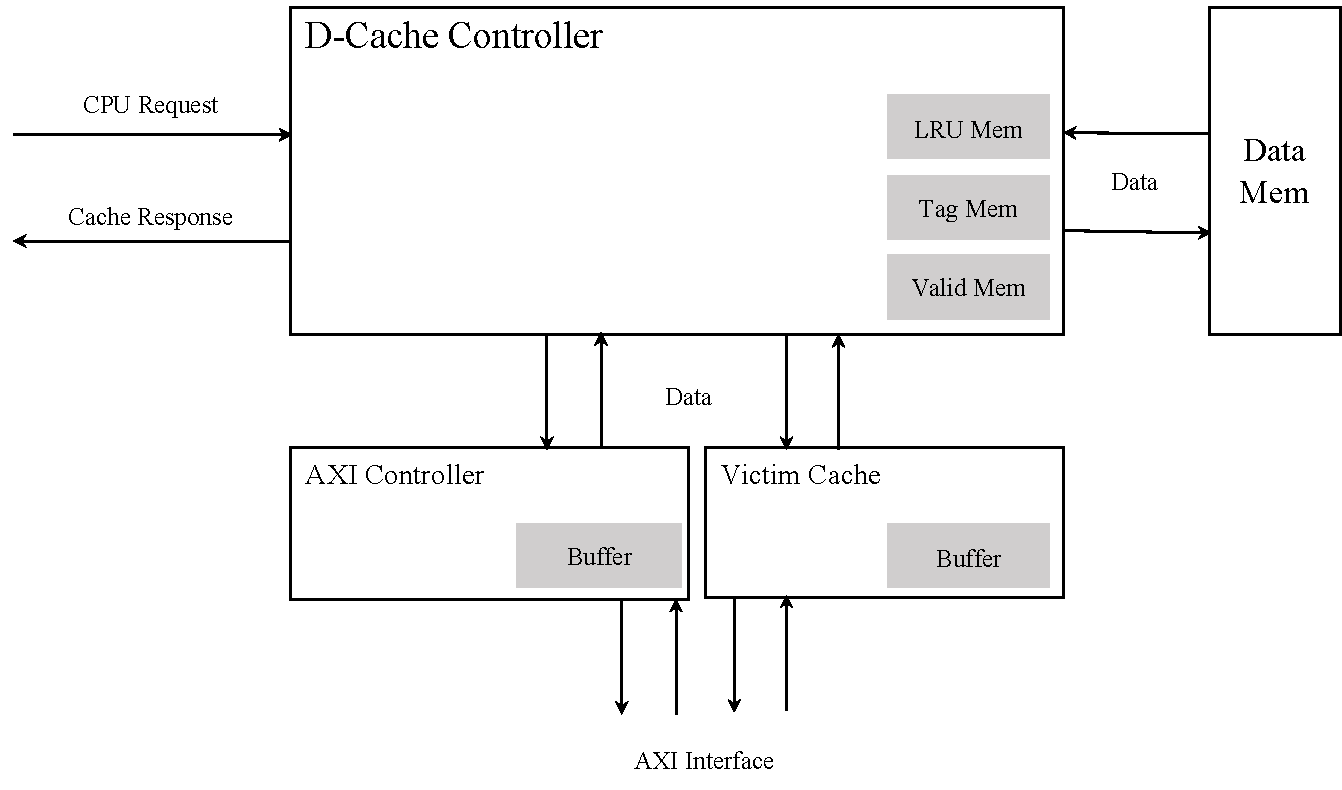
\includegraphics[width=\linewidth]{dcache.pdf}
	\caption{D-Cache结构}
	\label{fig:dcache}
\end{figure}

\subsection{写回缓存 (Victim Cache)}

Victim Cache能够处理D-Cache提交的写回请求。它的存在为Cache性能带来了两方面的提升,(1) D-Cache无需自行处理某一行的写回,无需等待写回完成就能进行新的AXI读取,减少了D-Cache的返回时延;(2) 当D-Cache发生 miss 时,若缺失的行为刚刚换出写回的行,则可以在一拍内从 Victim Cache 中获取,大大降低了在这种情况下的延迟。

Victim Cache本质是一个FIFO。当收到 D-Cache 发起的访存请求时,将该请求写入FIFO。AXI控制逻辑会按序完成FIFO中的写请求。只要FIFO没有被充满,Victim Cache都能立即响应D-Cache的请求。

值得注意的是,在FIFO中的每一行都有一个 valid 位,当写入请求时,valid 位被置为有效。当完成请求时,并不会清除 valid 位。而对于 D-Cache 的查询请求,所有 valid 位有效的行都能被命中。因而在 FIFO 中的数据,在完成写回之后,依然能够提供给D-Cache。这意味着在访存范围较大且前后反复访存导致写回频繁发生时,只要写回的行在重新命中时仍然在FIFO存储空间中未被覆盖,就能在一拍内返回给D-Cache,大大优化了性能。

然而,这也带来了一个问题:若同一行先后两次被提交进FIFO,则FIFO的存储空间中可能包含同一行的新旧两个版本。判断版本的新旧会带来较为复杂的逻辑,因而在我们的实现中,转而保证FIFO存储空间中任意时刻只可能有同一行的一个副本有效,且为最新的副本(如果有)。实现方法是在处理 D-Cache 的写回请求时,判断写回地址是否在FIFO存储空间中且有效,若有效则将其无效再将新请求的数据写入FIFO。

\begin{figure}[t]
	\centering
	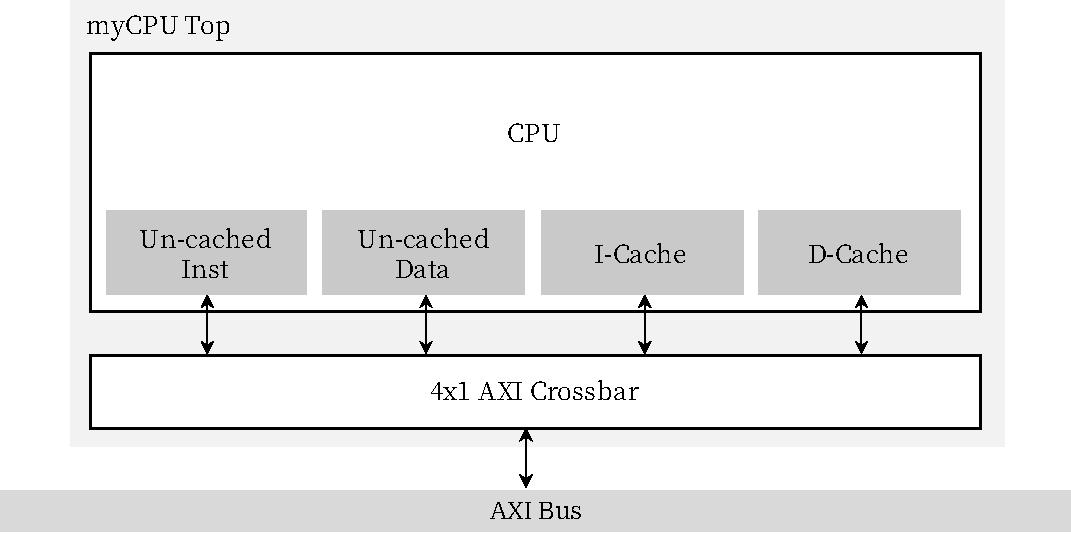
\includegraphics[width=0.7\linewidth]{cpu_interface.pdf}
	\caption{CPU外部接口}
	\label{fig:cpu-interface}
\end{figure}

\section{CPU外部接口}

CPU的整体结构如图 \ref{fig:cpu-interface} 中所示。CPU共引出了4个独立的AXI接口,分别是不经过缓存的取指、访存 (Un-cached Inst and Un-cached Data) 与经过缓存的取指、访存 (I-Cache and D-Cache)。由于提供SOC要求CPU仅仅引出一个AXI接口,因而使用Xilinx IP定制一个AXI Crossbar,包含4个 Slave Interface,一个 Master Interface,将四个AXI接口整合为一个引出到SOC。

而为了优化系统性能,采用了 \( \text{D-Cache} > \text{I-Cache} = \text{Un-cached Data} = \text{Un-cached Inst} \)的优先级配置,也即 D-Cache 访存优先级最高,其余三个进行公平竞争 (round-robin),来保证数据访存不会被其他请求阻塞。


	